\documentclass[conference]{IEEEtran}

% Packages
\usepackage[utf8]{inputenc}
\usepackage[english]{babel}
\usepackage{amsmath}
\usepackage{amsfonts}
\usepackage{amssymb}
\usepackage{amsthm}
\usepackage{pdfpages}
\usepackage{graphicx}
\usepackage{epstopdf}
\usepackage{listings}
\usepackage{cite}
\usepackage{enumerate}
\usepackage{scientific}
\usepackage[colorlinks=false]{hyperref}
\usepackage{bookmark}

\usepackage[]{mcode}	%Matlab Code
\usepackage{tikz,pgfplots}	%Tikz
\usepackage{paralist}	% Compact enum

\usepgfplotslibrary{external} 
\tikzexternalize
\tikzsetexternalprefix{ext/}

% Bookmark Setup
\bookmarksetup{numbered}

% PDF Setup
\hypersetup{pdftitle={Homework 5}, pdfsubject={Documentation of 5th Homework}, pdfauthor={Stefan Röhrl}, pdfkeywords={Neuroprothetik Exercise}, pdfcreator={LaTeX}, hidelinks}


\begin{document}
%
% cite all references
%\nocite{*}
%
% paper title
% can use linebreaks \\ within to get better formatting as desired
\title{Homework 5\\ Multicompartment Model}

\author{\IEEEauthorblockN{Stefan Röhrl}
\IEEEauthorblockA{Technische Universität München, Arcisstraße 21, Munich, Germany\\
Email: stefan.roehrl@tum.de}}

% use for special paper notices
%\IEEEspecialpapernotice{(Invited Paper)}

% make the title area
\maketitle

\IEEEpeerreviewmaketitle

\section{Create a Multicompartment Model}
Das Multicompartment Modell wurde durch Einfügen einer zusätzlichen Dimension in alle Variablen umgesetzt. Die neuen Spannungswerte werden wie in den Hausaufgaben Folien vorgeschlagen durch lösen eines Gleichungssystems berechnet.

\begin{lstlisting}
    % Berechnen Membranspannung
    B = V(:,k)+dt/c * (-sum(i_ion(:,k,:),3)...
        + iStimulus(:,k));
    A = (eye(comparts) - dt/(c * Ra) * C);
    V(:,k+1) = A\B;
\end{lstlisting}

\section{Experiments}

\begin{enumerate}

\item Die Anregung mit einem 5ms langen Puls mit einer Amplitude von $10\frac{\mu A}{cm^2}$ führt zu folgendem Verlauf der Membranpotentiale jedes Compartments. 

\begin{figure}[h]
	\centering
	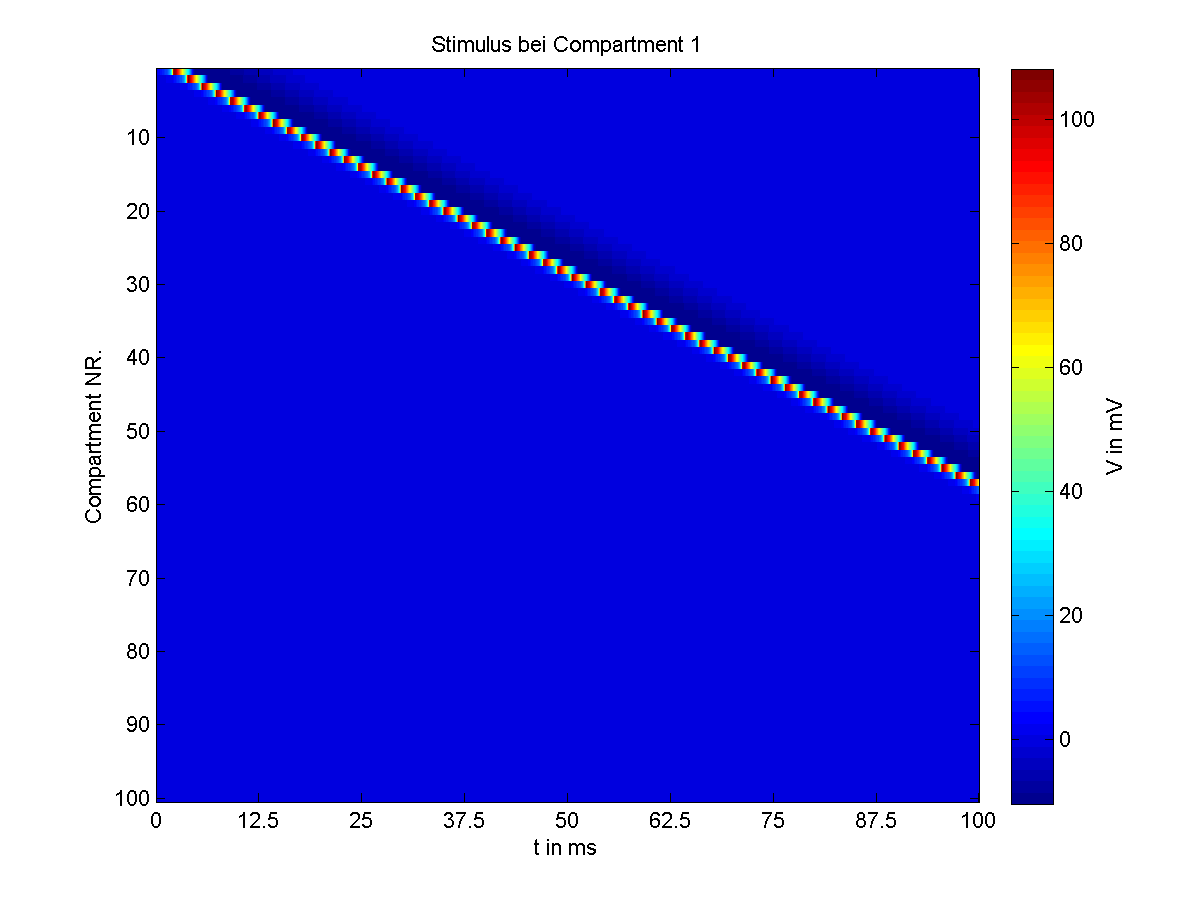
\includegraphics[width=0.5\textwidth]{img/compart1.png}
	\caption{Anregung an Compartment 1}
	\label{fig:compart1}
\end{figure}

\item Wenn man gleichzeitig Compartment 20 und 80 anregt, entstehen 4 sich fortbewegende Aktionspotentiale. Zwei laufen nach links und zwei nach rechts. Wenn ein Aktionspotential gerade ein Compartment passiert hat ist dieses Compartment refraktär und kann für eine bestimmte Zeit (Refraktärzeit) kein weiteres Aktionspotential mehr weiterleiten. Somit blockieren sich die aufeinander zulaufenden Aktionspotentiale gegenseitig und können sich nachdem sie sich begegnet sind nicht weiter laufen da in beide Richtungen die Compartments erst das entgegenkommende Aktionspotential weitergeleitet haben und somit kurzfristig kein neues Aktionspotential weiterleiten können.

\begin{figure}[h]
	\centering
	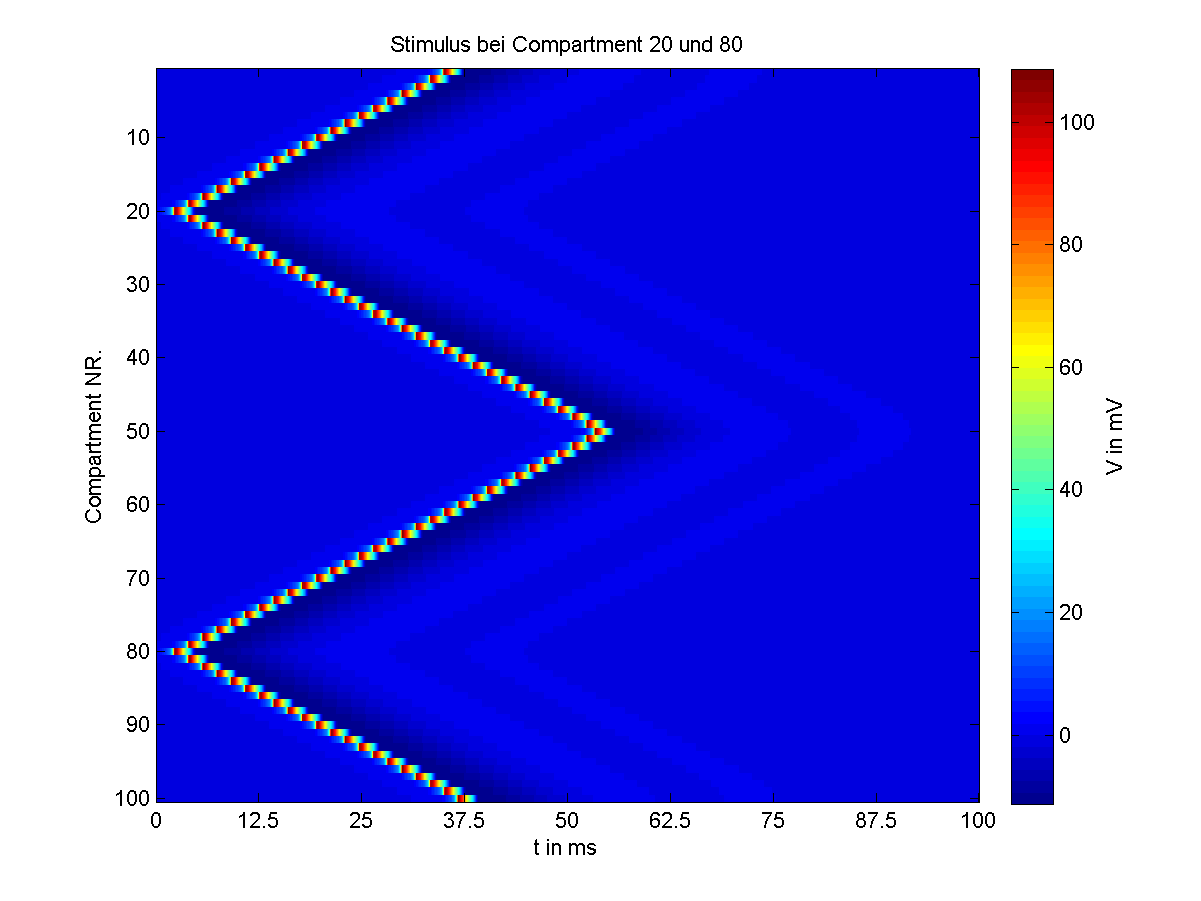
\includegraphics[width=0.5\textwidth]{img/compart20and80.png}
	\caption{Anregung an Compartment 20 und 80}
	\label{fig:compart20and80}
\end{figure}

\item In den folgenden Versuchen wurden die Parameter $c$ (Kapazität), $l_{comp}$ (Länge der Compartments), $r_{axon}$ (Radius des Axons), $\rho_{axon}$ (spezifischer Widerstand des Axons) und $T$ (Temperatur) geändert und die Auswirkungen auf den Verlauf des Aktionspotentials untersucht.\\
\begin{compactenum}[a)] 

\begin{figure}
	\centering
	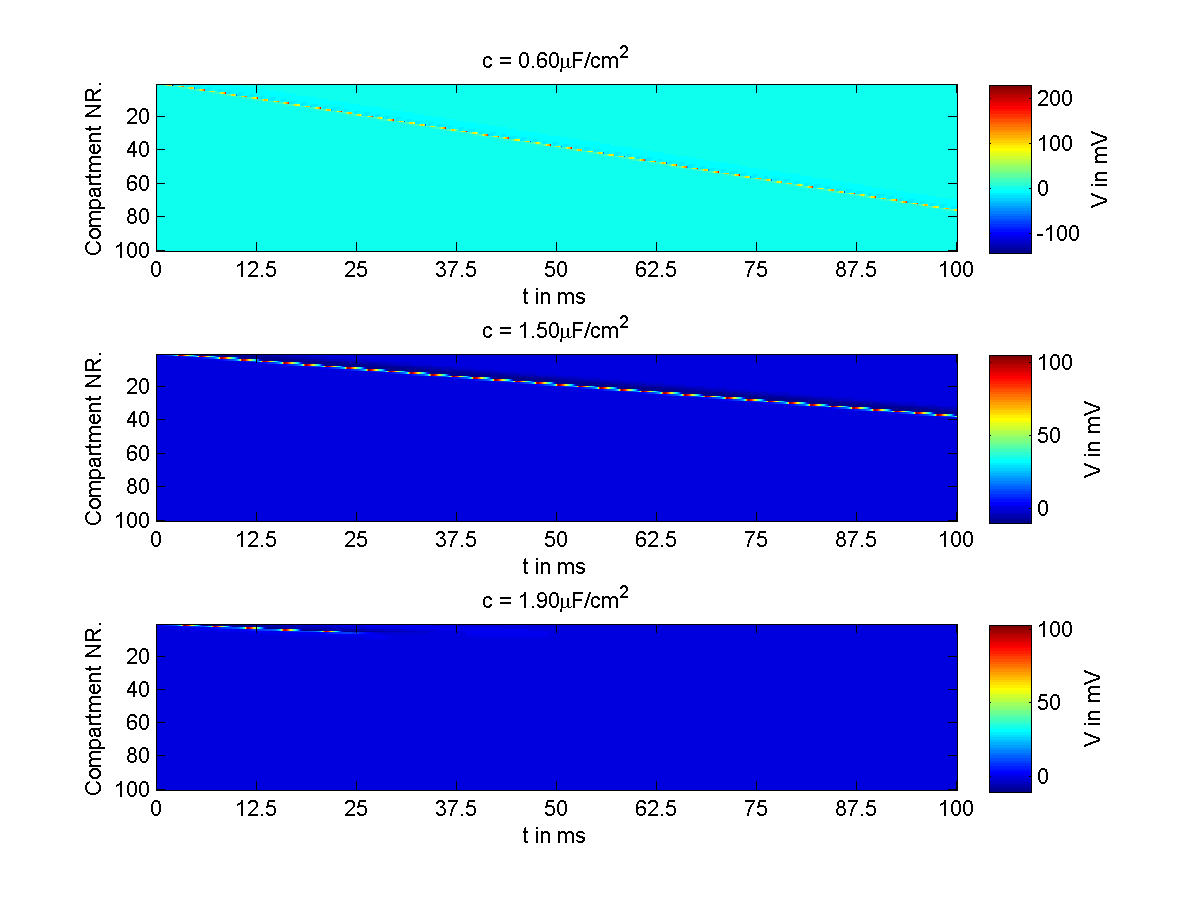
\includegraphics[width=0.5\textwidth]{img/change_c.png}
	\caption{Veränderung des Parameters $c = [0.60, 1.50, 1.90] \frac{\mu F}{cm^2}$}
	\label{fig:changec}
\end{figure}

\item Die Verringerung der Kapazität hat zur Folge, dass das Aktionspotential schneller durch die Compartments wandert. Die Zeit bis ein Aktionspotential ausgelöst wird ist kürzer da es nicht so lange dauert die Kapazität aufzuladen. Man kann auch beobachten, dass durch die kleinere Kapazität bei gleichem Strom eine höhere Spannung für das Aktionspotential erreicht wird. Jedoch ist auch die Überkompensation durch den Kalium-Strom größer und das Potential wird zwischenzeitlich negativer. Vergrößert man hingegen die Kapazität dauert es umso länger die Kapazität aufzuladen und das Aktionspotential propagiert langsamer. Ist die Kapazität zu groß reicht die Ladung (die durch die Leak-Ströme immer etwas kleiner wird) irgendwann nicht mehr aus, um ein Aktionspotential auszulösen und die Aktivierung endet. (vgl. Abb. \ref{fig:changec})\\

\begin{figure}
	\centering
	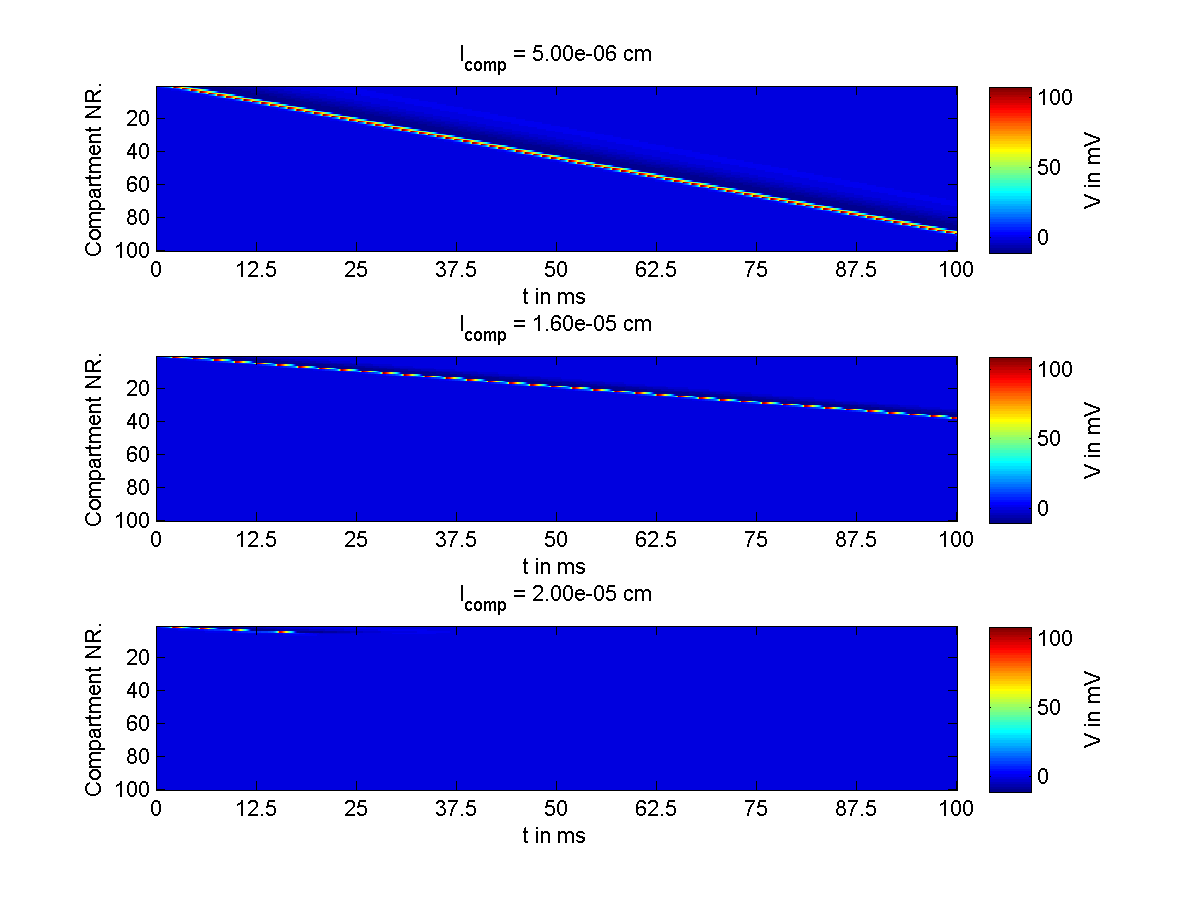
\includegraphics[width=0.5\textwidth]{img/change_l.png}
	\caption{Veränderung des Parameters $l_{comp} = [5.0e-6, 1.6e-5, 2.0e-5]cm$}
	\label{fig:changel}
\end{figure}

\item Je kürzer das Compartment ist, desto geringer ist sein Widerstand, da gilt: $R_a = \rho_{axon} \cdot \frac{l_{comp}}{r_{axon}^2}$ Daher kann bei einer kürzeren Compartment-Länge mehr Strom fließen und das Aktionspotential wird schneller erreicht. Somit propagiert das Aktionspotential schneller durch das Axon. Den gegenteiligen Effekt hat die Erhöhung der Axon-Länge. Ist das Axon zu lang ist der Widerstand zu groß und der Strom reicht nicht aus um die Membranspannung so weit ansteigen zu lassen, um ein Aktionspotential auszulösen. (vgl. Abb. \ref{fig:changel})\\

\begin{figure}
	\centering
	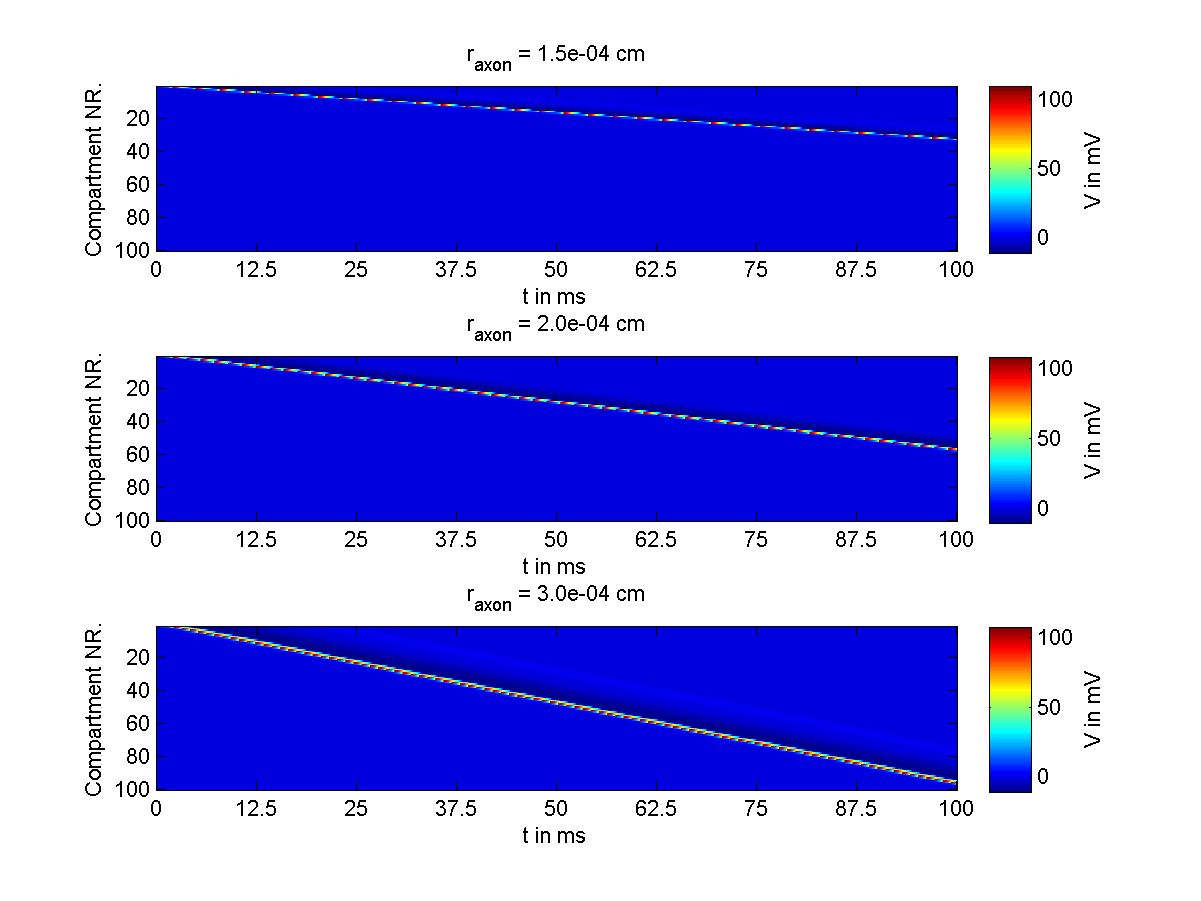
\includegraphics[width=0.5\textwidth]{img/change_r.png}
	\caption{Veränderung des Parameters $r_{axon} = [1.5, 2.0, 3.0] e-4cm$}
	\label{fig:changer}
\end{figure}

\item Die Veränderung des spezifischen Widerstands hat den selben Effekt wie die Veränderung der Compartment-Länge. Je geringer der spezifische Widerstand, desto schneller progagiert das Aktionspotential. Je höher der spezifische Widerstand desto langsamer ist es, bis es sogar ganz zum Stillstand kommt und nicht mehr weitergeleitet wird. (vgl. Abb. \ref{fig:changerho})\\

\begin{figure}
	\centering
	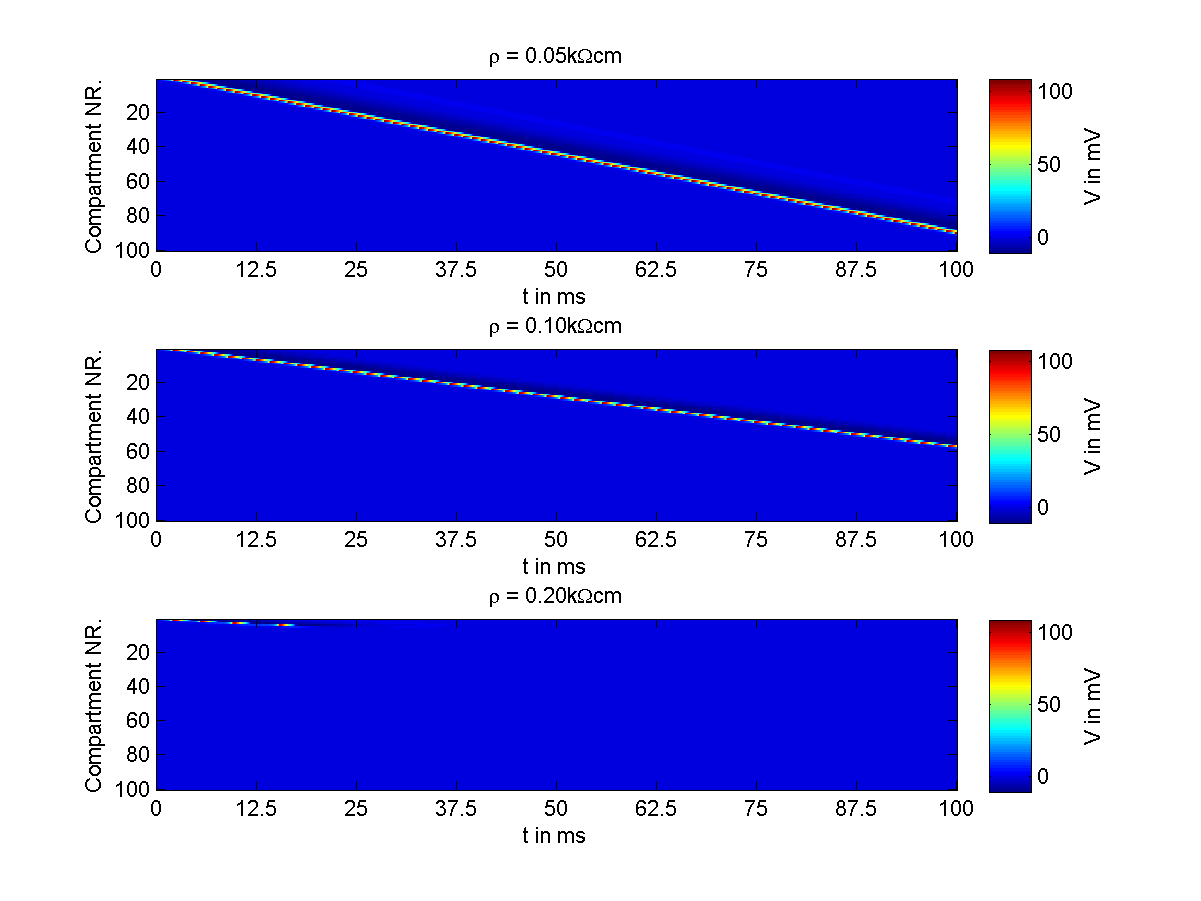
\includegraphics[width=0.5\textwidth]{img/change_rho.png}
	\caption{Veränderung des Parameters $\rho_{axon} = [0.05, 0.10, 0.20] k\Omega cm$}
	\label{fig:changerho}
\end{figure}

\item Da der Radius des Axons im Nenner steht wird die Leitfähigkeit des Axons mit steigendem Radius verbessert. Daher hat eine Veränderung des Radius eine umgekehrte Wirkung wie die Veränderung der Compartment-Länge oder des spezifischen Widerstandes. (Im Plot nicht abgebildet: Es kann auch hier zur Auslöschung des Aktionspotentials kommen, wenn der Radius zu klein gewählt wird.) (vgl. Abb. \ref{fig:changer})\\

\begin{figure}
	\centering
	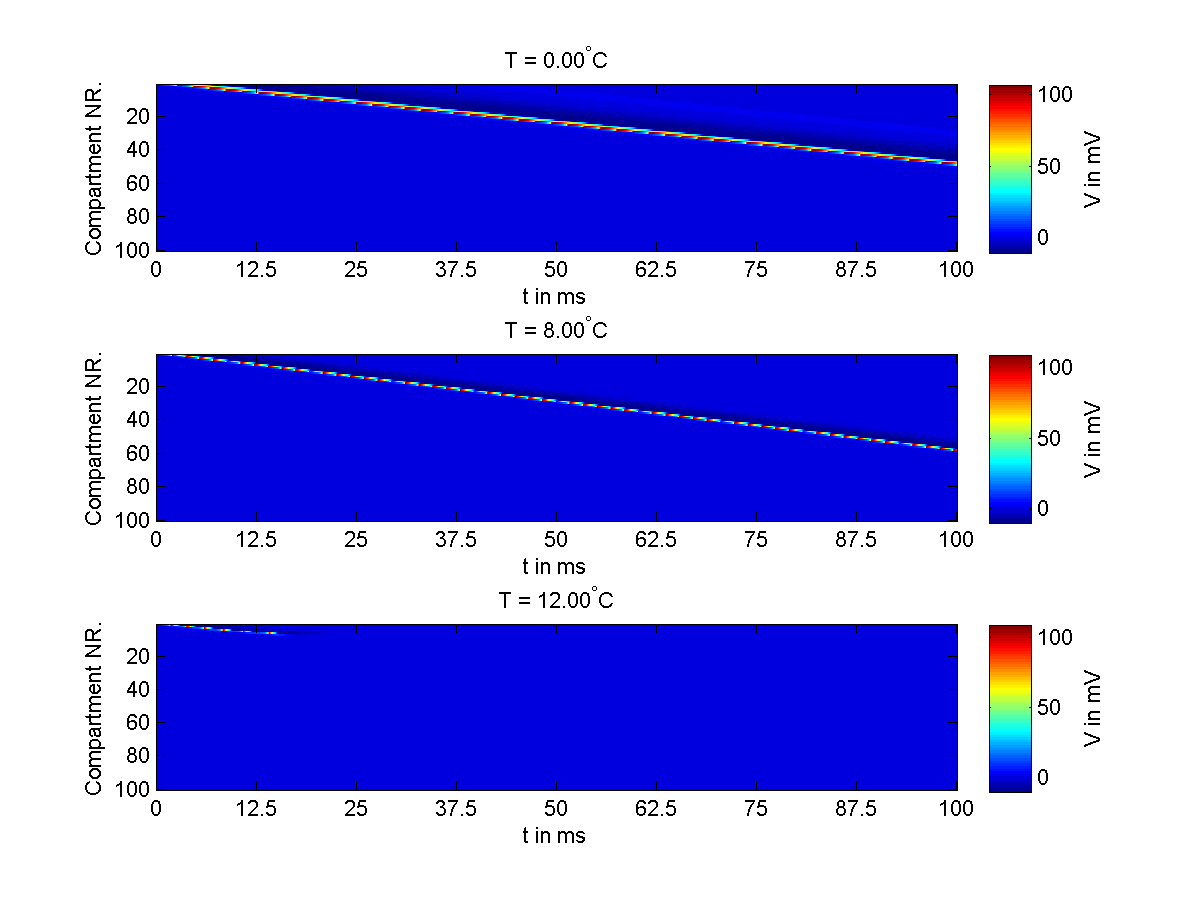
\includegraphics[width=0.5\textwidth]{img/change_T.png}
	\caption{Veränderung des Parameters $T = [0.00, 8.00, 12.00] ^\circ C$}
	\label{fig:changeT}
\end{figure}

\item Die Temperatur beeinflusst die Änderung der Gatting Variablen. Somit laufen die Reaktionen bei einer höheren Temperatur schneller ab. Dies sieht man auch in der Ausbreitung des Aktionspotentials. Bei niedrigerer Temperatur nahe $0^\circ$C kommt das Aktionspotential in 100ms nur bis Compartment 50. Bei höheren Temperaturen schon bis Compartment 60. Ist die Temperatur zu hoch (ab ca. 12 $^\circ$C) funktioniert das Differentialgleichungssystem nicht mehr. Man sieht zwar, dass am Anfang das Aktionspotential sehr schnell weitergeleitet wird, jedoch komm es nach ein paar Compartments zum Erliegen. (vgl. Abb. \ref{fig:changeT})\\

\end{compactenum}

\end{enumerate}

\end{document}


